\documentclass[aspectratio=169]{beamer}
\usepackage[utf8]{inputenc}
\usepackage{lmodern}
\usepackage{tikz}
\usepackage{hyperref}
\hypersetup{hidelinks}
\usetikzlibrary{positioning,arrows.meta,calc}

\definecolor{accent1}{HTML}{0F766E}
\definecolor{accent2}{HTML}{99F6E4}
\definecolor{accent3}{HTML}{F59E0B}
\definecolor{accent4}{HTML}{134E4A}
\definecolor{paper}{HTML}{F7FEFC}
\definecolor{ink}{HTML}{1F2937}

\setbeamertemplate{navigation symbols}{}
\setbeamercolor{normal text}{fg=ink,bg=white}
\setbeamercolor{frametitle}{fg=ink,bg=white}
\setbeamertemplate{itemize item}{\color{accent1}$\blacktriangleright$}
\setbeamertemplate{enumerate item}{\color{accent1}\insertenumlabel.}
\setbeameroption{hide notes}

\title{Lesson 2: Build Step by Step}
\subtitle{MagicSchool Student Project Guide}
\author{Pine Brook IGNITE}
\date{Spring 2026}

\begin{document}

\begin{frame}[plain]
\begin{tikzpicture}[remember picture,overlay]
\fill[paper] (current page.south west) rectangle (current page.north east);
\fill[accent1!10] (0.25,0.4) rectangle (13.05,7.0);
\draw[line width=7pt, color=accent3] (0.55,6.75) -- (12.75,6.75);
\draw[line width=7pt, color=accent2] (0.55,0.65) -- (12.75,0.65);
\end{tikzpicture}
\vspace{0.45cm}
\begin{columns}[T,totalwidth=\textwidth]
\column{0.57\textwidth}
{\huge\bfseries\color{ink} Lesson 2: Build Step by Step\par}
\vspace{0.2cm}
{\Large\color{accent4} Use your guide. Build one part at a time.\par}
\vspace{0.25cm}

\begin{tikzpicture}
\node[rounded corners=16pt, fill=white, draw=accent1, line width=1.2pt, text width=6.4cm, minimum height=1.35cm, align=center]
{\Large\bfseries AI helps us build. We stay in charge.};
\end{tikzpicture}
\vspace{0.35cm}
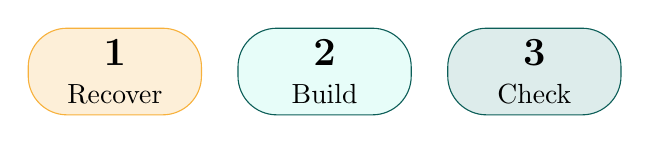
\begin{tikzpicture}[node distance=0.45cm]
\node[rounded corners=14pt, fill=accent3!16, draw=accent3!80, minimum width=2.2cm, minimum height=1.1cm, align=center] (a) {\Large\bfseries 1\\[2pt]Recover};
\node[rounded corners=14pt, fill=accent2!24, draw=accent1!80!black, minimum width=2.2cm, minimum height=1.1cm, align=center, right=of a] (b) {\Large\bfseries 2\\[2pt]Build};
\node[rounded corners=14pt, fill=accent1!14, draw=accent1!80!black, minimum width=2.2cm, minimum height=1.1cm, align=center, right=of b] (c) {\Large\bfseries 3\\[2pt]Check};
\end{tikzpicture}
\column{0.38\textwidth}
\begin{center}
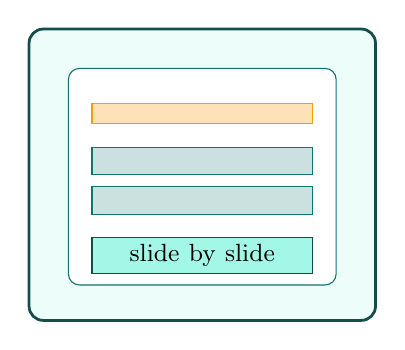
\begin{tikzpicture}[x=1cm,y=1cm]
\draw[rounded corners=0.18cm, fill=accent2!18, draw=accent4, line width=1pt] (0.4,0.5) rectangle (4.8,4.2);
\draw[rounded corners=0.14cm, fill=white, draw=accent1] (0.9,0.95) rectangle (4.3,3.7);
\draw[fill=accent3!30, draw=accent3] (1.2,3.0) rectangle (4.0,3.25);
\draw[fill=accent1!22, draw=accent1] (1.2,2.35) rectangle (4.0,2.7);
\draw[fill=accent1!22, draw=accent1] (1.2,1.85) rectangle (4.0,2.2);
\draw[fill=accent2!90, draw=accent4] (1.2,1.1) rectangle (4.0,1.55);
\node[text width=2.3cm, align=center] at (2.6,1.33) {\small slide by slide};
\end{tikzpicture}
\end{center}
\end{columns}
\note{Open with the new mission: students are building, not planning from scratch.}
\end{frame}

\begin{frame}[plain]
\frametitle{Today's Mission}
\begin{block}{By the end of Lesson 2, I will have:}
\begin{itemize}
\large
\item my topic and guide recovered or confirmed
\item 2 to 3 built sections or slides
\item a project that still fits my CS goal
\item a clear next step for Lesson 3
\end{itemize}
\end{block}
\vspace{0.15cm}
\begin{center}
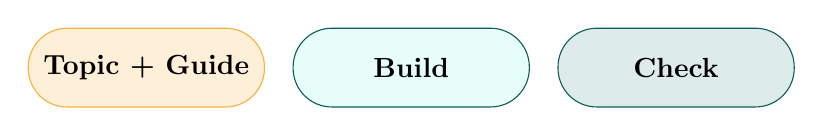
\begin{tikzpicture}[node distance=0.35cm]
\node[rounded corners=14pt, fill=accent3!16, draw=accent3!80, minimum width=3.0cm, minimum height=1.0cm, align=center] (a) {\bfseries Topic + Guide};
\node[rounded corners=14pt, fill=accent2!24, draw=accent1!80!black, minimum width=3.0cm, minimum height=1.0cm, align=center, right=of a] (b) {\bfseries Build};
\node[rounded corners=14pt, fill=accent1!14, draw=accent1!80!black, minimum width=3.0cm, minimum height=1.0cm, align=center, right=of b] (c) {\bfseries Check};
\end{tikzpicture}
\end{center}
\end{frame}

\begin{frame}[plain]
\frametitle{Quick Re-Entry}
\begin{block}{Before you start building, check 4 things}
\begin{enumerate}
\large
\item My topic is:
\item My project type is:
\item My guide has 3 to 5 parts:
\item My topic still connects to computer science:
\end{enumerate}
\end{block}
\vspace{0.15cm}
\begin{block}{If you are missing one of these}
\large Use the AI Assistant with teacher help to recover it quickly, then start building.
\end{block}
\end{frame}

\begin{frame}[plain]
\frametitle{Our AI Rules}
\begin{columns}[T,totalwidth=\textwidth]
\column{0.54\textwidth}
\begin{itemize}
\large
\item Do not type names or private information.
\item AI is a helper, not the boss.
\item AI can be wrong.
\item We choose what to keep or change.
\item The teacher can see class AI work.
\end{itemize}
\column{0.4\textwidth}
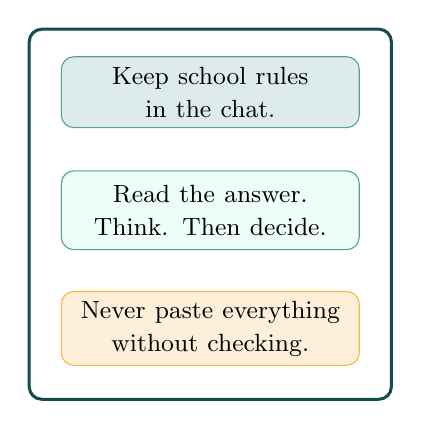
\begin{tikzpicture}[x=1cm,y=1cm]
\draw[rounded corners=0.16cm, fill=white, draw=accent4, line width=1.1pt] (0.1,0.1) rectangle (4.7,4.8);
\node[rounded corners=0.16cm, fill=accent1!14, draw=accent1!70, text width=3.55cm, minimum height=0.9cm, align=center] at (2.4,4.0) {\small Keep school rules in the chat.};
\node[rounded corners=0.16cm, fill=accent2!18, draw=accent1!70, text width=3.55cm, minimum height=1.0cm, align=center] at (2.4,2.5) {\small Read the answer. Think. Then decide.};
\node[rounded corners=0.16cm, fill=accent3!16, draw=accent3!75, text width=3.55cm, minimum height=0.9cm, align=center] at (2.4,1.0) {\small Never paste everything without checking.};
\end{tikzpicture}
\end{columns}
\end{frame}

\begin{frame}[plain]
\frametitle{Today's Tools}
\begin{columns}[T,totalwidth=\textwidth]
\column{0.48\textwidth}
\begin{block}{AI Assistant}
\begin{itemize}
\large
\item Recover a guide if needed
\item Clarify one part
\item Turn one part into notes
\item Check your section
\end{itemize}
\end{block}
\column{0.48\textwidth}
\begin{block}{Project Tool}
\begin{itemize}
\large
\item Build your slideshow
\item One section at a time
\item Use your guide
\item Save your work
\end{itemize}
\end{block}
\end{columns}
\vspace{0.15cm}
\begin{center}
\Large\bfseries AI Assistant first if stuck. Project tool for the real work.
\end{center}
\end{frame}

\begin{frame}[plain]
\frametitle{Our Workflow}
\begin{center}
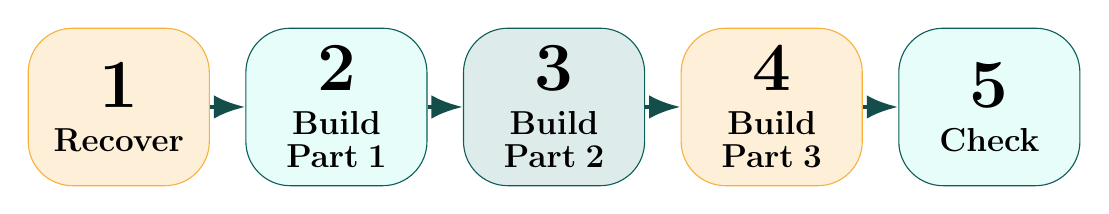
\begin{tikzpicture}[node distance=0.45cm]
\node[rounded corners=16pt, fill=accent3!16, draw=accent3!80, minimum width=2.3cm, minimum height=2.0cm, text width=1.8cm, align=center] (s1) {\Huge\bfseries 1\\[4pt]\large Recover};
\node[rounded corners=16pt, fill=accent2!24, draw=accent1!80!black, minimum width=2.3cm, minimum height=2.0cm, text width=1.8cm, align=center, right=of s1] (s2) {\Huge\bfseries 2\\[4pt]\large Build Part 1};
\node[rounded corners=16pt, fill=accent1!14, draw=accent1!80!black, minimum width=2.3cm, minimum height=2.0cm, text width=1.8cm, align=center, right=of s2] (s3) {\Huge\bfseries 3\\[4pt]\large Build Part 2};
\node[rounded corners=16pt, fill=accent3!16, draw=accent3!80, minimum width=2.3cm, minimum height=2.0cm, text width=1.8cm, align=center, right=of s3] (s4) {\Huge\bfseries 4\\[4pt]\large Build Part 3};
\node[rounded corners=16pt, fill=accent2!24, draw=accent1!80!black, minimum width=2.3cm, minimum height=2.0cm, text width=1.8cm, align=center, right=of s4] (s5) {\Huge\bfseries 5\\[4pt]\large Check};
\draw[-{Latex[length=4mm,width=3mm]}, line width=1.7pt, color=accent4] (s1) -- (s2);
\draw[-{Latex[length=4mm,width=3mm]}, line width=1.7pt, color=accent4] (s2) -- (s3);
\draw[-{Latex[length=4mm,width=3mm]}, line width=1.7pt, color=accent4] (s3) -- (s4);
\draw[-{Latex[length=4mm,width=3mm]}, line width=1.7pt, color=accent4] (s4) -- (s5);
\end{tikzpicture}
\end{center}
\vspace{0.25cm}
\begin{block}{Remember}
\large Build first. Decorate later.
\end{block}
\end{frame}

\begin{frame}[plain]
\frametitle{AI Assistant Prompt Cards}
\begin{block}{Use the AI Assistant to build from your guide}
\begin{itemize}
\large
\item My topic is \_\_\_\_. Part 1 of my guide is \_\_\_\_. Give me 3 to 5 notes or bullet points I can use on one slide.
\item My topic is \_\_\_\_. Here is my draft section: \_\_\_\_. Does it match my guide and my computer science goal?
\item My topic is \_\_\_\_. Help me explain this part in clear Grade 4 language: \_\_\_\_.
\item My topic is \_\_\_\_. What details are missing from this part of my project: \_\_\_\_?
\end{itemize}
\end{block}
\vspace{0.2cm}
\begin{center}
\Large\bfseries Use one prompt at a time, then build the real section yourself.
\end{center}
\end{frame}

\begin{frame}[plain]
\frametitle{Worked Example}
\begin{columns}[T,totalwidth=\textwidth]
\column{0.48\textwidth}
\begin{block}{Topic and Guide}
\begin{itemize}
\large
\item Topic: How robots help animals
\item Part 1: What robots are
\item Part 2: Ways robots help animals
\item Part 3: Why this matters
\end{itemize}
\end{block}
\column{0.48\textwidth}
\begin{block}{One Real Slide}
\begin{itemize}
\large
\item Slide title: Ways robots help animals
\item Bullet 1: Robots can help scientists watch animals safely.
\item Bullet 2: Robots can help rescue or care for animals.
\item Bullet 3: Robots use code and sensors to do jobs.
\end{itemize}
\end{block}
\end{columns}
\vspace{0.15cm}
\begin{block}{What happened here?}
\large The guide turned into one real section. That is the goal for today.
\end{block}
\end{frame}

\begin{frame}[plain]
\frametitle{What Not To Do}
\begin{columns}[T,totalwidth=\textwidth]
\column{0.48\textwidth}
\begin{block}{Do}
\begin{itemize}
\large
\item use your guide first
\item build one section at a time
\item ask AI for help with one part
\item check if it still fits your topic
\end{itemize}
\end{block}
\column{0.52\textwidth}
\begin{block}{Do Not}
\begin{itemize}
\large
\item start decorating before building
\item paste the whole AI answer
\item skip your guide
\item forget the CS connection
\end{itemize}
\end{block}
\end{columns}
\end{frame}

\begin{frame}[plain]
\frametitle{Midpoint Checklist}
\begin{itemize}
\large
\item I have my topic and guide.
\item I built Part 1.
\item I built Part 2.
\item I am working on Part 3.
\item My project still matches my computer science goal.
\item I know what I still need to do next.
\end{itemize}
\vspace{0.2cm}
\begin{block}{If you are stuck}
\large Guide first. One small step. Partner. One AI prompt. Then teacher.
\end{block}
\end{frame}

\begin{frame}[plain]
\frametitle{Ready for Lesson 3?}
\begin{block}{Before you leave, make sure you can say:}
\begin{itemize}
\large
\item What topic are you building?
\item Which sections did you finish today?
\item How did AI help without taking over?
\item What still needs work before Lesson 3?
\end{itemize}
\end{block}
\vspace{0.2cm}
\begin{center}
\Large\bfseries Save your work. Be ready to revise and finish next time.
\end{center}
\end{frame}

\end{document}
